\section{Understanding word2vec (Refresher)}
Let's have a quick refresher on the {\tt word2vec} algorithm. The key insight behind {\tt word2vec} is that \textit{`a word is known by the company it keeps'}. Concretely, suppose we have a `center' word $c$ and a contextual window surrounding $c$. We shall refer to words that lie in this contextual window as `outside words'. For example, in Figure~\ref{fig:word2vec} we see that the center word $c$ is `banking'. Since the context window size is 2, the outside words are `turning', `into', `crises', and `as'. \newline

The goal of the skip-gram {\tt word2vec} algorithm is to accurately learn the probability distribution $P(O \vert C)$. Given a specific word $o$ and a specific word $c$, we want to calculate $P(O=o \vert C=c)$, which is the probability that word $o$ is an `outside' word for $c$, i.e., the probability that $o$ falls within the contextual window of $c$.

\begin{figure}[h]
    \centering
    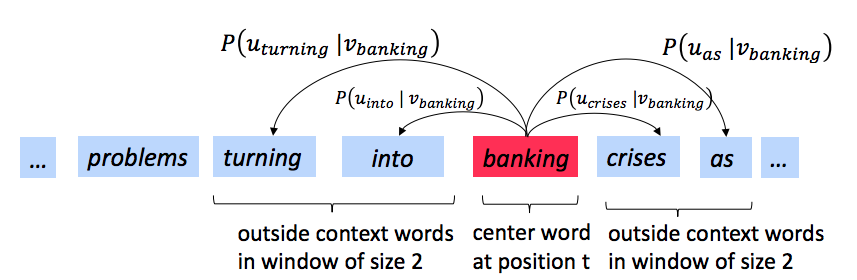
\includegraphics[width=\textwidth]{word2vec.png}
    \caption{The word2vec skip-gram prediction model with window size 2}\label{fig:word2vec}
\end{figure}

In {\tt word2vec}, the conditional probability distribution is given by taking vector dot-products and applying the softmax function: % I added the word "softmax" here because I bet a lot of students will have forgotten what softmax is and why the loss fn is called naive softmax. but if this is too wordy we can just take it out

\begin{equation}
 P(O=o \vert C=c) = \frac{\exp(\bm{u_{o}^{\top} v_c})}{\sum_{w \in \text{Vocab}} \exp(\bm{u_{w}^{\top} \bm v_c})} % NUMERATOR: \exp(\bm u_{o}^\top \bm v_c) %DENOMINATOR: \sum_{w \in \text{Vocab}} \exp(\bm u_{w}^\top \bm v_c)
 \label{word2vec_condprob}
\end{equation}

Here, $\bm u_o$ is the `outside' vector representing outside word $o$, and $\bm v_c$ is the `center' vector representing center word $c$. 
To contain these parameters, we have two matrices, $\bm U$ and $\bm V$.
The columns of $\bm U$ are all the `outside' vectors $\bm u_{w}$. 
The columns of $\bm V$ are all of the `center' vectors $\bm v_{w}$. 
Both $\bm U$ and $\bm V$ contain a vector for every $w \in \text{Vocabulary}$.\footnote{Assume that every word in our vocabulary is matched to an integer number $k$.  $\bm u_{k}$ is both the $k^{th}$ column of $\bm U$ and the `outside' word vector for the word indexed by $k$. $\bm v_k$ is both the $k^{th}$ column of $\bm V$ and the `center' word vector for the word indexed by $k$. \textbf{In order to simplify notation we shall interchangeably use $k$ to refer to the word and the index-of-the-word.}}\newline

%We can think of the probability distribution $P(O|C)$ as a prediction function that we can approximate via supervised learning. For any training example, we will have a single $o$ and $c$. We will then compute a value $P(O=o|C=c)$ and report the loss. 
Recall from lectures that, for a single pair of words $c$ and $o$, the loss is given by:

\begin{equation} 
\bm J_{\text{naive-softmax}}(\bm v_c, o, \bm U) = -\log P(O=o \vert C=c).
\label{naive-softmax}
\end{equation}

Another way to view this loss is as the cross-entropy\footnote{The Cross Entropy Loss between the true (discrete) probability distribution $p$ and another distribution $q$ is $-\sum_i p_i \log(q_i)$.} between the true distribution $\bm y$ and the predicted distribution $\hat{\bm y}$. 
Here, both $\bm y$ and $\hat{\bm y}$ are vectors with length equal to the number of words in the vocabulary.
Furthermore, the $k^{th}$ entry in these vectors indicates the conditional probability of the $k^{th}$ word being an `outside word' for the given $c$. 
The true empirical distribution $\bm y$ is a one-hot vector with a 1 for the true outside word $o$, and 0 everywhere else. 
The predicted distribution $\hat{\bm y}$ is the probability distribution $P(O \vert C=c)$ given by our model in equation (\ref{word2vec_condprob}). There are 2 optional questions below which you may attempt (\emph{Note: Bonus points will be awarded for the optional assignments})

\begin{enumerate}[(a)]
    \item \points{1a} \textbf{Extra Credit Challenge I} \newline
        The partial derivative of $\bm J_{\text{naive-softmax}}(\bm v_c, o, \bm U)$ with respect to $\bm v_c$ in terms of  $\bm y$, $\hat{\bm y}$, and $\bm U$ is given below:
        \begin{equation}
            {\partial J \over \partial \bm v_c} = \bm U(\hat{\bm y} - \bm y) 
        \end{equation}
        or equivalently,
        \begin{equation}
            {\partial J \over \partial \bm v_c} = -\bm u_o + \sum_{w=1}^{V} \hat{y}_w \bm u_w  
        \end{equation}

        The naive-softmax loss given in Equation (\ref{naive-softmax}) is the same as the cross-entropy loss between $\bm y$ and $\hat{\bm y}$; This is equivalent to:

        \begin{equation} 
        -\sum_{w \in Vocab} y_w \log(\hat{y}_w) = - \log (\hat{y}_o).
        \end{equation}
        \newline
        Since $\bm y$ is a one-hot vector, all $\bm y_{k} = 0$ where $k \neq o$. $\bm y_o$ = 1, so we are left with $- \log (\hat{\bm{y}}_o)$.
        \\[0.5in]
        \textbf{Write the steps} to arrive at equation 3 or 4, the partial derivative of $\bm J_{\text{naive-softmax}}(\bm v_c, o, \bm U)$ with respect to $\bm v_c$, starting from equation 5. Please write your answer in terms of $\bm y$, $\hat{\bm y}$, and $\bm U$. The first few steps have been provided below (loss function $\bm J_{\text{naive-softmax}}(\bm v_c, o, \bm U)$) and the rest of the proof may take 4 or 5 steps.

        \begin{align*}
            J_{\text{naive-softmax}}(\bm v_c, o, \bm U) &= - \log (\hat{y}_o) &&\text{(refer to equation 5)}\\
            &= -\log \bigg( \frac{\exp(\bm u_{o}^\top \bm v_c)}{\sum_{w \in \text{Vocab}} \exp(\bm u_{w}^\top \bm v_c)} \bigg) \\
            &= -\bigg( \log\big(\exp(\bm u_{o}^\top \bm v_c)\big) - \log \big( \sum_{w \in \text{Vocab}} \exp(\bm u_{w}^\top \bm v_c) \big) \bigg) \\
            &= - \bm u_{o}^\top \bm v_c + \log \big( \sum_{w \in \text{Vocab}} \exp(\bm u_{w}^\top \bm v_c) \big)     
        \end{align*}
    \item \points{1b} \textbf{Extra Credit Challenge II} \newline
        The partial derivatives of $\bm J_{\text{naive-softmax}}(\bm v_c, o, \bm U)$ with respect to each of the `outside' word vectors, $\bm u_w$'s is given below:

        \begin{equation}
            {\partial J \over \partial \bm U } = {\bm v_c} (\hat{\bm y} - \bm y)^\top    
        \end{equation}
        or equivalently:
        \begin{align}
            {\partial J\over \partial \bm u_w} = 
            \begin{cases}
                (\hat{y}_w-1) {\bm v_c} & \text{if } w=o \\
            \hat{y}_w{\bm v_c} & \text{otherwise}
            \end{cases}
        \end{align}
    
        \textbf{Write the steps} required to arrive at the partial derivative of $\bm J_{\text{naive-softmax}}(\bm v_c, o, \bm U)$ with respect to each of the `outside' word vectors, $\bm u_w$'s. There are two cases you need to consider: when $w=o$, the true `outside' word vector, and $w \neq o$, for all other words. Please write you answer in terms of $\bm y$, $\hat{\bm y}$, and $\bm v_c$. The proof may take 4 or 5 steps. The loss function $\bm J_{\text{naive-softmax}}(\bm v_c, o, \bm U)$ is:

            \begin{equation*}
            J_{\text{naive-softmax}}(\bm v_c, o, \bm U) = - \bm u_{o}^\top \bm v_c + \log \bigg( \sum_{w' \in \text{Vocab}} \exp(\bm u_{w'}^\top \bm v_c) \bigg)
            \end{equation*}
\end{enumerate}